\documentclass[11pt,a4paper]{article}

\usepackage[utf8]{inputenc}
\usepackage[T1]{fontenc}
\usepackage{lmodern}
\usepackage[margin=2.5cm]{geometry}
\usepackage{graphicx}
\usepackage{booktabs}
\usepackage{tabularx}
\usepackage{array}
\usepackage[font=small]{caption}
\usepackage{url}
\usepackage[hidelinks]{hyperref}

\renewcommand{\arraystretch}{1.15}
\newcolumntype{L}{>{\raggedright\arraybackslash}X}
\setlength{\parskip}{0.5em}
\setlength{\parindent}{0pt}
\graphicspath{{figures/}}
\renewcommand{\topfraction}{0.9}
\renewcommand{\bottomfraction}{0.8}
\renewcommand{\textfraction}{0.1}
\renewcommand{\floatpagefraction}{0.8}

\begin{document}

\begin{center}
{\Large Data-quality controls with and without AI}\\[0.4em]
{\large What two pilot studies showed}\\[0.8em]
Tomash Oosterbaan\\
MSc Artificial Intelligence, University of Groningen\\
Graduation project context: Avanade and Rabobank\\
October 2026
\end{center}

\section{Starting point}

Data from a new source is rarely ready for use. Before a bank uses it in reports, models or decisions, a data team checks it with validation rules: required fields must be present, values must have the right type, codes must come from an agreed list. Long Tran described this work in his context at Rabobank as technical validation, business rules, monitoring thresholds and manual investigation of exceptions \cite{tran}. A public Rabobank case study also names missing data and differences between information providers as practical problems \cite{alderse}. The team then faces a question: is it worth adding something smarter on top of these checks, such as a statistical model or AI, and how would it know?

This report describes how we explored that question in two pilot studies and a short follow-up. The first pilot tested error detectors on public tables. Its results led to a second pilot, in which AI writes validation rules that are tested against rules written by experts. A mini-pilot then checked the weakest points of the second pilot. All data is public; no Rabobank data is used.

One method runs through all of this: controlled error injection. We take real data, change values in a copy on purpose and record exactly what we changed. Because we know where the errors are, we can measure which errors a control finds, which it misses and how many false alarms it raises. Changed values are not proof of real-world errors, so each pilot also looked for real errors where it could.

\section{Pilot 1: which error detector should a team choose?}

\subsection{The idea}

My first proposal was about choosing an error detector. There are many methods, from rules and statistics to learned detectors such as CDC, which predicts each value from the other columns and flags values that do not fit \cite{cdc}, or LUCARIO, which learns common formats and ranges from the data \cite{lucario}. How well they work depends on the errors. Jung et al.\ separate the type of an error, what happens to a value, from its mechanism, which values are affected \cite{taberr}. Table~\ref{tab:mech} shows the three mechanisms.

\begin{table}[htbp]
\centering
\small
\begin{tabularx}{\textwidth}{@{}p{1.4cm}LL@{}}
\toprule
Mechanism & Which values are affected & Example \\
\midrule
ECAR & Completely at random & A random selection of monthly bills is multiplied by ten. \\
EAR & Depends on another field & The errors occur mainly in records from one source system. \\
ENAR & Depends on the value itself & Large bills are more likely to be multiplied by ten. \\
\bottomrule
\end{tabularx}
\caption{Error mechanisms after Jung et al.\ \cite{taberr}. The change itself stays the same; only its placement differs.}
\label{tab:mech}
\end{table}

Detectors are usually compared on random errors (ECAR). The idea was that a detector chosen that way might be the wrong choice when errors cluster in one source system or in large amounts. We wanted to compare that usual choice with a mechanism-aware choice: the detector with the best result under its weakest mechanism. The CURED demonstrator, which combines this error model with CDC, was the starting point \cite{cured}.

\subsection{What we did}

We used three public tables from the UCI repository: credit card clients (30{,}000 rows), the closest public equivalent of a bank credit file \cite{uci-credit}; bank marketing (41{,}188 rows), with many categorical fields \cite{uci-bank}; and white wine quality (4{,}898 rows), to see whether results hold outside finance \cite{uci-wine}. Each table had 800 evaluation rows and separate historical rows to learn what normal data looks like.

We injected five types of errors: missing values, wrong data types, invalid codes, amounts multiplied by ten, and plausible substitutions (a valid value replaced by another valid value). Each was applied to 1, 5 or 10\% of a column, under all three mechanisms, with five repetitions: 630 scenarios. A second round of 360 scenarios focused on errors that pass basic rules, such as a bill copied from the wrong month.

The baseline was what a team already has: rules for required fields, types and allowed codes, simple statistical checks learned from history (unusual ranges, rare categories), and later simple prediction models (Ridge and logistic regression). On top of that we tested CDC, dBoost, LUCARIO, RIOLU \cite{riolu}, Auto-Test \cite{autotest}, Raha \cite{raha} and a small experiment inspired by ZeroED, in which a language model helps label values \cite{zeroed}. We measured not only how many injected errors a detector finds, but how many it finds that the baseline misses, how many extra alerts it creates, and what is left when a reviewer can check only 20 alerts per 800 rows. That last measure follows Abedjan et al., who showed that extra tools find more errors but also produce more alerts that a person has to check \cite{abedjan}.

\subsection{What we found}

First, the rules caught every missing value, wrong type and invalid code. Advanced detectors only matter for errors that pass the rules.

Second, the mechanism changed how much a detector added, but not which detector was best (Figure~\ref{fig:mech}). For amounts multiplied by ten in the credit table, CDC found 23\% extra changed values when errors were placed at random, 14\% when they clustered in one group and 27\% when they hit large amounts. The other detectors added almost nothing under any mechanism, and in the wine table no detector added anything. With one detector on top wherever anything worked, there was little left to select.

\begin{figure}[htbp]
\centering
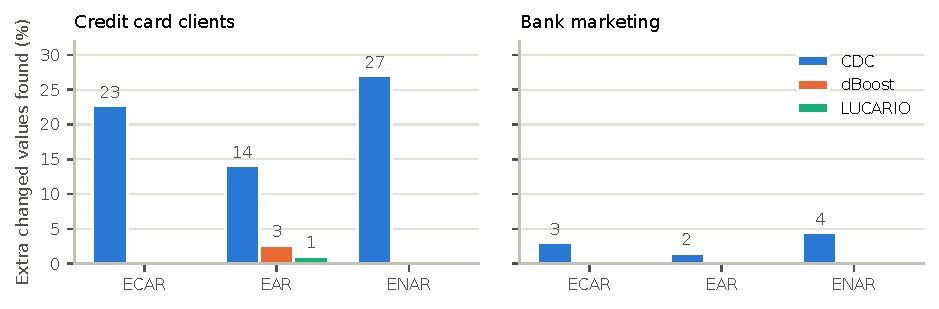
\includegraphics[width=\textwidth]{fig_a_mechanism.pdf}
\caption{Pilot 1. Changed values found beyond rules and statistical checks, for amounts multiplied by ten in 5\% of a column, by mechanism. Mean of five runs. In the wine table no detector added anything.}
\label{fig:mech}
\end{figure}

Third, the extra findings came at a high price (Figure~\ref{fig:inc}). For errors that pass the rules, CDC found 11 to 21 of 40 changed values that rules, statistics and a Ridge model missed, but added 520 to 900 alerts per batch. With 20 reviews per batch, the net gain was $+0.4$ changed values for Bank, $0$ for Credit and $-1.0$ for Wine, and a simple logistic regression removed the small gain for Bank. On published benchmarks, Auto-Test added 4 to 5 correct findings at 25 reviews, and none if the existing alerts were reviewed first. Where a copy of the original source existed, simply comparing source and copy found every change.

\begin{figure}[htbp]
\centering
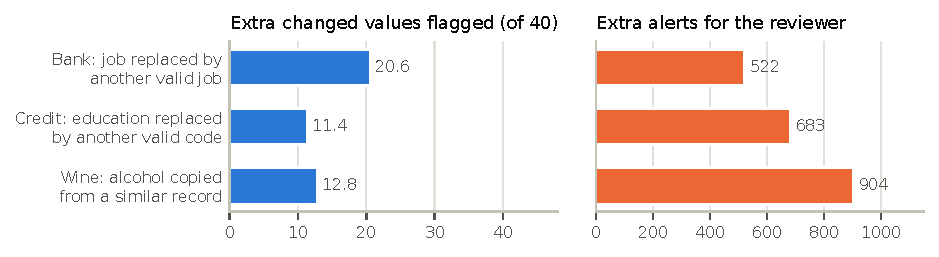
\includegraphics[width=\textwidth]{fig_a_increment.pdf}
\caption{Pilot 1. CDC added to rules, statistical checks and a Ridge model, for errors that pass the rules; 5\% changed values, random placement, mean of five runs.}
\label{fig:inc}
\end{figure}

\subsection{Why we moved on}

The selection question did not hold up: the mechanism mattered for the size of the effect, not for the choice. The remaining question, what an extra detector adds beyond existing controls when review time is limited, had already been studied \cite{abedjan,rein}, so the room for a new contribution was small. All errors were made by us, and AI played only a minor role. Two lessons went into the next pilot: always compare with strong, cheap baselines, and always report the alerts next to the findings.

\section{Pilot 2: can AI-written rules be trusted?}

\subsection{The idea}

Instead of a model that flags values, AI can write rules. An analyst asks a language model for checks and receives readable rules within seconds. For a bank this is attractive, because a rule can be read, approved and audited, which is harder for a detector. Recent studies do exactly this \cite{ledqer,akella,audq}, and data-quality tools are starting to offer it \cite{rehberger}. These studies judge the generated rules against labelled data or human ratings. The AuDQ authors note that their datasets have no ``reference rule set to compare against'' \cite{audq}, and Alexander et al.\ compared generated tests with one suite written by one data scientist \cite{alexander}. There are also reasons for caution: automatically discovered rules are mostly false \cite{martin}, and language models give different code on different runs \cite{ouyang}.

Our idea was to test AI-written rules against a large public set of expert rules with official test cases, and to reuse the injection method of pilot 1 as a stress test for both the expert rules and the AI rules. Injecting errors to test checks has been done before \cite{homayouni,jenga}; using it to compare AI rules with an expert rule set had not.

\subsection{Data: financial filings and the DQC rules}

American listed companies file their reports with the SEC in XBRL, a machine-readable format in which every number is a separate fact with a standard label, a period, a unit and a precision. For example: \texttt{Revenues} $=$ 5{,}000{,}000, for 2024, in US dollars, rounded to thousands. The Data Quality Committee (DQC) of XBRL US publishes about 200 free rules that find common mistakes in these filings, such as assets that do not equal liabilities plus equity, or amounts that should never be negative \cite{dqc}. Each rule has a written description, an official implementation that runs in the open-source program Arelle \cite{arelle}, and official test cases: example filings with the exact messages the rule should give. These test cases work as an answer key. Each rule also has a release date, so we can tell which rules a model could have seen during its training.

When a company finds a mistake, it can file an amended report; comparing the two shows which numbers changed. Such amendments have been used as signals of misreporting before \cite{brown}. We used the SEC Financial Statement Data Sets for 2023 to mid-2025 (68{,}875 filings, 1{,}294 original and amended pairs) \cite{fsds}, 240 XBRL filings (120 never corrected, 120 later corrected) and version 31 of the DQC rules.

\subsection{What we did}

The existing controls were generic checks, three statistical checks learned from filings outside the sample (unusual sign, unusual size, unusual jump between periods), a deliberately naive rule that amounts are never negative, and the official DQC rules. We injected seven types of errors into the filings: a flipped sign, a value multiplied by 1{,}000, a changed amount, one changed digit, a wrong element, swapped periods and a removed fact, with sizes based on the real corrections.

Two small open-source models, Qwen2.5-Coder-7B and Qwen3-8B \cite{qwen25coder,qwen3}, ran on a normal processor: free, no data leaves the machine, and the release date is known. They wrote rules in three ways: from the description of a DQC rule, from a sample of a filing, and from a list of error types that the existing controls missed. All generated code ran in a sandbox. As a comparison, a model also acted as a judge that reads a filing and points at suspicious numbers. AI rules were only evaluated on filings no model had seen. Before running anything we fixed an approval gate: at most one alert per filing that was never corrected, at least 20\% of the missed errors caught, and the same result when the rule is generated again.

\subsection{What we found}

Reproducing expert rules. For rules released before the models, both models found about 41\% of the official messages; for rules released after them, 3\% and 13\% (Figure~\ref{fig:e1}). Most rules scored 0\%, a few close to 100\%. A rule we translated by hand found 15 of 16 messages, so the test setup was not the cause. Writing the same rule three times often gave very different results, for two rules anywhere from 0\% to 100\%.

\begin{figure}[htbp]
\centering
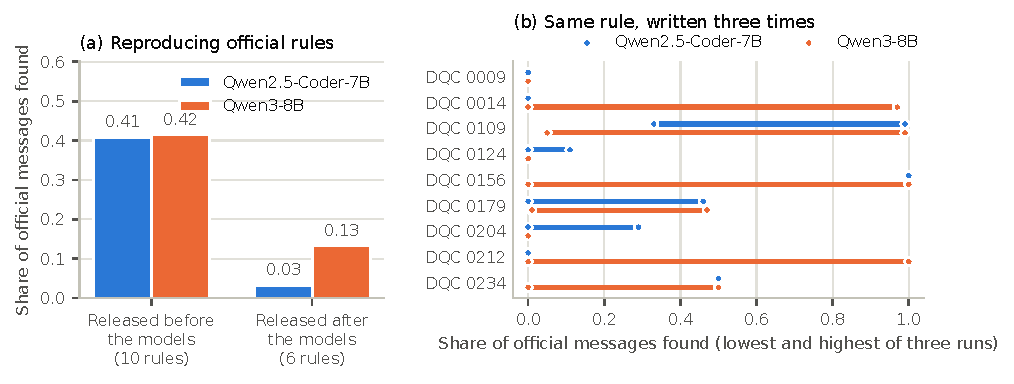
\includegraphics[width=\textwidth]{fig_b_e1_e5.pdf}
\caption{Pilot 2. (a) Share of official DQC messages found by rules the models wrote from the rule descriptions. (b) Lowest and highest result of three generations of the same rule.}
\label{fig:e1}
\end{figure}

Injected errors. The statistical checks caught two thirds of the x1000 errors and little else. The DQC rules caught 17 to 64\% per error type, but no removed facts. Together, the existing controls caught 27 of 83 injected errors, about a third. The best AI rule set caught 6 more, but gave on average 458 alerts on a filing that was never corrected, against 1.8 for DQC and 0.1 to 2.6 for each statistical check (Figure~\ref{fig:alerts}). None of the AI rule sets passed the gate. The alerts came from domain mistakes rather than programming mistakes: one rule compared the period type of each fact, stored as ``instant'', with a list that codes it as ``I'', and another assumed that elements with a debit balance can never be negative, which is not true in XBRL \cite{debreceny}. The AI judge caught 2 of 42 injected errors; it could see only 19 of them, and caught 2 of those.

\begin{figure}[htbp]
\centering
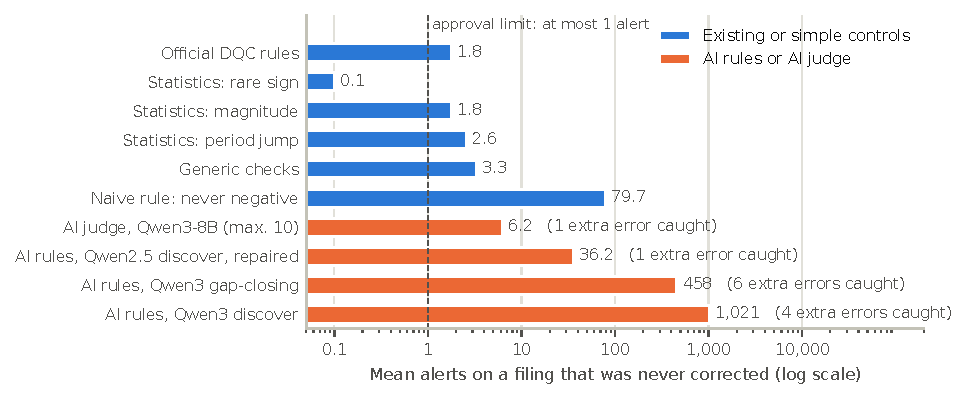
\includegraphics[width=\textwidth]{fig_b_alerts.pdf}
\caption{Pilot 2. Mean alerts on test filings that were never corrected (66 filings; DQC on 12; AI judge on 6). In brackets: injected errors caught beyond the existing controls. Log scale.}
\label{fig:alerts}
\end{figure}

Real corrections. Most amendments were accounting restatements, not typing errors. I checked 20 targeted corrections against the documents, starting from labels that an AI model had pre-filled: the original number was wrong in 9 cases (7 restatements and 2 tagging errors), not wrong in 3 and unclear in 8. Two separate AI passes over the same items agreed on only half of them. On later-corrected numbers, DQC flagged 1.6\% and the statistical checks 0.1 to 0.6\%. Real corrections are therefore useful as candidates, but not yet as a gold standard.

\section{Mini-pilot: checking the weak points}

Three short checks addressed the main doubts about pilot 2. First, none of the 66 test filings shares a company with a filing used for development, so the results are not inflated by overlap. Second, we gave one model the official implementation of nine rules it had failed. Three then worked, one of them exactly, on a rule released after the model; one found all messages but also about 3{,}300 others. The other six still failed: three on carrying the logic over to the data, two on information that only the taxonomy holds, and one on a programming error. Missing documentation therefore explains only a small part of the failures.

Third, we looked at the 24 single sub-rules inside the AI rule sets instead of judging each set as a whole. We chose sub-rules on half of the test filings and measured on the other half (Figure~\ref{fig:qual}). Without filtering, they caught 42 of the 195 errors the existing controls missed, at about 1{,}000 alerts per filing. Keeping only sub-rules that add something beyond the existing controls, within one alert per filing, left one sub-rule that caught 3 extra errors at 0.2 alerts. A generic filter that ignores the existing controls needed about twice as many alerts for the same gain. Most extra catches were sign errors. Alert limits above 1 and 5 were chosen after seeing the first results, so that part is exploratory.

\begin{figure}[htbp]
\centering
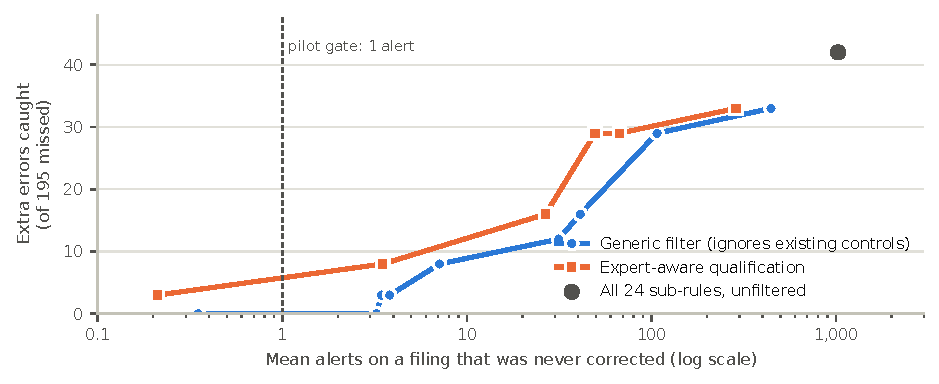
\includegraphics[width=\textwidth]{fig_c_qualification.pdf}
\caption{Mini-pilot. Extra injected errors caught beyond the existing controls (of 195 missed) against mean alerts per filing, on the evaluation half (34 filings). Each point is a set of sub-rules chosen on the other half under an alert limit.}
\label{fig:qual}
\end{figure}

\section{What we learned and where this leads}

Four lessons hold across both pilots. Strong, cheap baselines matter: rules caught all hard errors in pilot 1, statistical checks catch scale errors in pilot 2, and a simple model erased the gain of an advanced detector. Alerts decide usefulness: in both pilots, extra findings came with hundreds of alerts. Injected errors are needed to measure anything, but real corrections are mostly accounting changes that data-quality rules are not designed for. And with small models, AI-written rules are unstable and add little, but selecting single rules against the existing controls is a measurable step that separates useful from noisy rules.

This points to a thesis question about that selection step: under what conditions can LLM-generated validation rules be qualified to add reliable detection value beyond expert-defined controls, and at what review cost? Answering it requires larger open-weight models on the university GPU cluster, more DQC rules with the official implementation as a separate condition, comparison of AI and official rules on the same real filings, a sample of real corrections judged by two people with XBRL or accounting knowledge, and two to four further public datasets that come with their own expert rules, such as European ESEF reports, GLEIF entity records and HMDA mortgage data \cite{esef,gleif,hmda}.

The pilots also produced a working tool, \texttt{dqstress}, that follows the steps of a data team onboarding a source. It runs the existing controls, stress-tests them with injected errors, lets a local model propose rules for the gaps, tests each proposal in a sandbox against the approval gate, and records the human decision with the evidence. It does not change data and never approves a rule by itself. In the thesis it would be extended with the per-rule qualification from the mini-pilot.

\begin{thebibliography}{99}
\small
\setlength{\itemsep}{2pt}
\setlength{\parskip}{0pt}

\bibitem{tran} L. Tran, correspondence with the author, 4 September 2026 (unpublished; observations specific to his working context).

\bibitem{alderse} T. Alderse Baas, ``A Real-Life Machine Learning Journey,'' Rabobank Techblog, 15 September 2021. \url{https://rabobank.jobs/en/techblog/a-real-life-machine-learning-journey/}

\bibitem{cdc} S. J\"ager and F. Biessmann, ``From Data Imputation to Data Cleaning: Automated Cleaning of Tabular Data Improves Downstream Predictive Performance,'' Proceedings of AISTATS, PMLR 238, pp. 3394--3402, 2024.

\bibitem{lucario} Q. Qin, H. Li, and E. Merlo, ``Unsupervised, Robust, and Lightweight Detection of Data Pattern Anomalies and Outliers,'' Information and Software Technology, vol. 192, article 108035, 2026. doi:10.1016/j.infsof.2026.108035.

\bibitem{taberr} P. Jung, S. J\"ager, N. Chandler, and F. Biessmann, ``Towards Realistic Error Models for Tabular Data,'' ACM Journal of Data and Information Quality, vol. 17, no. 4, article 28, 2025. doi:10.1145/3774914.

\bibitem{cured} N. Chandler, S. J\"ager, P. Jung, and F. Bie{\ss}mann, ``CURED: Creating, Understanding, and Repairing Errors Demonstrator,'' arXiv:2607.20140, 2026.

\bibitem{uci-credit} I.-C. Yeh, ``Default of Credit Card Clients,'' UCI Machine Learning Repository, 2009. doi:10.24432/C55S3H.

\bibitem{uci-bank} S. Moro, P. Rita, and P. Cortez, ``Bank Marketing,'' UCI Machine Learning Repository, 2014. doi:10.24432/C5K306.

\bibitem{uci-wine} P. Cortez, A. Cerdeira, F. Almeida, T. Matos, and J. Reis, ``Wine Quality,'' UCI Machine Learning Repository, 2009. doi:10.24432/C56S3T.

\bibitem{riolu} Q. Qin, H. Li, E. Merlo, and M. Lamothe, ``Automated, Unsupervised, and Auto-Parameterized Inference of Data Patterns and Anomaly Detection,'' Proceedings of ICSE, pp. 2419--2431, 2025. doi:10.1109/ICSE55347.2025.00078.

\bibitem{autotest} Q. Chen, Y. He, R. C.-W. Wong, W. Cui, S. Ge, H. Zhang, D. Zhang, and S. Chaudhuri, ``Auto-Test: Learning Semantic-Domain Constraints for Unsupervised Error Detection in Tables,'' Proceedings of the ACM on Management of Data, vol. 3, no. 3, 2025. doi:10.1145/3725396.

\bibitem{raha} M. Mahdavi, Z. Abedjan, R. C. Fernandez, S. Madden, M. Ouzzani, M. Stonebraker, and N. Tang, ``Raha: A Configuration-Free Error Detection System,'' Proceedings of SIGMOD, pp. 865--882, 2019. doi:10.1145/3299869.3324956.

\bibitem{zeroed} W. Ni, K. Zhang, X. Miao, X. Zhao, Y. Wu, Y. Wang, and J. Yin, ``ZeroED: Hybrid Zero-Shot Error Detection Through Large Language Model Reasoning,'' Proceedings of ICDE, pp. 3126--3139, 2025. doi:10.1109/ICDE65448.2025.00234.

\bibitem{abedjan} Z. Abedjan, X. Chu, D. Deng, R. C. Fernandez, I. F. Ilyas, M. Ouzzani, P. Papotti, and M. Stonebraker, ``Detecting Data Errors: Where are we and what needs to be done?,'' Proceedings of the VLDB Endowment, vol. 9, no. 12, pp. 993--1004, 2016. doi:10.14778/2994509.2994518.

\bibitem{rein} M. Abdelaal, C. Hammacher, and H. Schoening, ``REIN: A Comprehensive Benchmark Framework for Data Cleaning Methods in ML Pipelines,'' Proceedings of EDBT, pp. 499--511, 2023. arXiv:2302.04702.

\bibitem{ledqer} A.-C. Glock, T. H\"utter, J. F\"urnkranz, W. W\"o{\ss}, A. Dominka-Kiss, and L. Ehrlinger, ``Data Quality Rule Generation with LLMs,'' arXiv:2609.06053, 2026.

\bibitem{akella} A. Akella, A. Kaul, K. Narayanam, and S. Mehta, ``Quality Assessment of Tabular Data using Large Language Models and Code Generation,'' Proceedings of EMNLP 2025: Industry Track, pp. 2713--2748, 2025. doi:10.18653/v1/2025.emnlp-industry.183.

\bibitem{audq} J. Biggiogera, N. Colombo, K. Saxena, B. Sarmah, and S. Pasquali, ``AuDQ: Auditable Data Quality through Agentic Rule Discovery,'' arXiv:2610.26031, 2026.

\bibitem{rehberger} T. Rehberger, T. H\"utter, L. Ehrlinger, and W. W\"o{\ss}, ``Evaluating Data Quality Tools: Measurement Capabilities and LLM Integration,'' arXiv:2604.09163, 2026.

\bibitem{alexander} R. Alexander, L. Katz, C. Moore, M. W.-C. Wong, and Z. Schwartz, ``Evaluating the Decency and Consistency of Data Validation Tests Generated by LLMs,'' arXiv:2310.01402, 2023.

\bibitem{martin} A. Martin, E. C. de Almeida, O. Romero, and A. Queralt, ``How and Why False Denial Constraints are Discovered,'' Proceedings of the VLDB Endowment, vol. 18, no. 10, pp. 3477--3489, 2025. doi:10.14778/3748191.3748209.

\bibitem{ouyang} S. Ouyang, J. M. Zhang, M. Harman, and M. Wang, ``An Empirical Study of the Non-Determinism of ChatGPT in Code Generation,'' ACM Transactions on Software Engineering and Methodology, vol. 34, no. 2, 2025. doi:10.1145/3697010.

\bibitem{homayouni} H. Homayouni, S. Ghosh, and I. Ray, ``An Approach for Testing the Extract-Transform-Load Process in Data Warehouse Systems,'' Proceedings of IDEAS, pp. 236--245, 2018. doi:10.1145/3216122.3216149.

\bibitem{jenga} S. Schelter, T. Rukat, and F. Biessmann, ``JENGA: A Framework to Study the Impact of Data Errors on the Predictions of Machine Learning Models,'' Proceedings of EDBT, pp. 529--534, 2021.

\bibitem{dqc} XBRL US Data Quality Committee, ``DQC rules (dqc\_us\_rules),'' rules, documentation and test suite, version 31. \url{https://github.com/DataQualityCommittee/dqc_us_rules}

\bibitem{arelle} Arelle, open-source XBRL platform, version 2.47.3. \url{https://arelle.org}

\bibitem{brown} N. C. Brown, R. M. Crowley, and W. B. Elliott, ``What Are You Saying? Using Topic to Detect Financial Misreporting,'' Journal of Accounting Research, vol. 58, no. 1, pp. 237--291, 2020. doi:10.1111/1475-679X.12294.

\bibitem{fsds} U.S. Securities and Exchange Commission, ``Financial Statement Data Sets,'' quarters 2023q1 to 2025q2. \url{https://www.sec.gov/data-research/sec-markets-data/financial-statement-data-sets}

\bibitem{qwen25coder} B. Hui, J. Yang, Z. Cui, J. Yang, et al., ``Qwen2.5-Coder Technical Report,'' arXiv:2409.12186, 2024.

\bibitem{qwen3} A. Yang, A. Li, B. Yang, B. Zhang, et al., ``Qwen3 Technical Report,'' arXiv:2505.09388, 2025.

\bibitem{debreceny} R. Debreceny, S. Farewell, M. Piechocki, C. Felden, and A. Gr\"aning, ``Does it add up? Early evidence on the data quality of XBRL filings to the SEC,'' Journal of Accounting and Public Policy, vol. 29, no. 3, pp. 296--306, 2010. doi:10.1016/j.jaccpubpol.2010.04.001.

\bibitem{esef} XBRL International, ``filings.xbrl.org,'' public repository of ESEF filings. \url{https://filings.xbrl.org}

\bibitem{gleif} Global Legal Entity Identifier Foundation, ``Data Quality Management,'' including the Data Quality Rule Setting. \url{https://www.gleif.org/en/lei-data/gleif-data-quality-management/}

\bibitem{hmda} Federal Financial Institutions Examination Council and Consumer Financial Protection Bureau, ``Filing Instructions Guide for HMDA data collected in 2024.'' \url{https://ffiec.cfpb.gov/documentation/fig/2024/overview}

\end{thebibliography}

\end{document}
